\documentclass[tikz, border=4pt]{standalone}

\usepackage{amsmath,amssymb}
\usetikzlibrary{arrows.meta, calc}
\usepackage{xcolor}

\definecolor{utnblue}{RGB}{0, 51, 102}
\definecolor{utnred}{RGB}{204, 0, 0}

\begin{document}
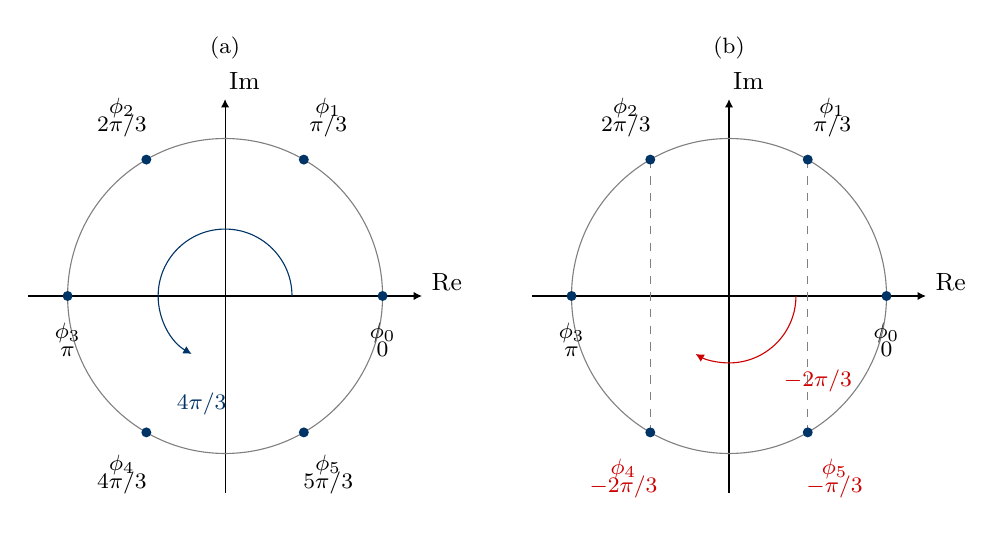
\begin{tikzpicture}[>={Latex[length=3pt,width=3pt]}, font=\small]

    \def\R{2.0}
    \def\D{6.4}

    % ==========================================================
    % (a) las frecuencias contadas de 0 a 2pi
    % ==========================================================
    \begin{scope}
        \draw[->, thin, black] (-\R-0.5,0) -- (\R+0.5,0) node[right, yshift=5pt] {$\operatorname{Re}$};
        \draw[->, thin, black] (0,-\R-0.5) -- (0,\R+0.5) node[above, xshift=7pt] {$\operatorname{Im}$};
        \draw[thin, gray] (0,0) circle (\R);

        % arco que mide lambda_4, hacia adelante
        \draw[utnblue, thin, ->] (0.85,0) arc (0:240:0.85);
        \node[utnblue, font=\footnotesize, anchor=north] at (255:1.15) {$4\pi/3$};

        \foreach \a/\k/\lam in {60/1/{$\pi/3$}, 120/2/{$2\pi/3$},
                                240/4/{$4\pi/3$}, 300/5/{$5\pi/3$}} {
            \fill[utnblue] (\a:\R) circle (1.8pt);
            \node[font=\footnotesize, align=center] at (\a:\R+0.62)
                 {$\phi_{\k}$\\[-3pt]\lam};
        }

        \foreach \a/\k/\lam in {0/0/{$0$}, 180/3/{$\pi$}} {
            \fill[utnblue] (\a:\R) circle (1.8pt);
            \node[font=\footnotesize, align=center, anchor=north] at ($(\a:\R)+(0,-0.22)$)
                 {$\phi_{\k}$\\[-3pt]\lam};
        }

        \node[font=\footnotesize] at (0,\R+1.15) {(a)};
    \end{scope}

    % ==========================================================
    % (b) las mismas frecuencias reducidas a (-pi, pi]
    % ==========================================================
    \begin{scope}[xshift=\D cm]
        \draw[->, thin, black] (-\R-0.5,0) -- (\R+0.5,0) node[right, yshift=5pt] {$\operatorname{Re}$};
        \draw[->, thin, black] (0,-\R-0.5) -- (0,\R+0.5) node[above, xshift=7pt] {$\operatorname{Im}$};
        \draw[thin, gray] (0,0) circle (\R);

        % pares conjugados, espejados en el eje real
        \draw[gray, thin, dashed] (60:\R) -- (300:\R);
        \draw[gray, thin, dashed] (120:\R) -- (240:\R);

        % arco que mide lambda_4 reducida, hacia atras
        \draw[utnred, thin, ->] (0.85,0) arc (0:-120:0.85);
        \node[utnred, font=\footnotesize, anchor=north west] at (-55:1.0) {$-2\pi/3$};

        \foreach \a/\k/\lam in {60/1/{$\pi/3$}, 120/2/{$2\pi/3$}} {
            \fill[utnblue] (\a:\R) circle (1.8pt);
            \node[font=\footnotesize, align=center] at (\a:\R+0.62)
                 {$\phi_{\k}$\\[-3pt]\lam};
        }
        \foreach \a/\k/\lam in {240/4/{$-2\pi/3$}, 300/5/{$-\pi/3$}} {
            \fill[utnblue] (\a:\R) circle (1.8pt);
            \node[font=\footnotesize, align=center, text=utnred] at (\a:\R+0.68)
                 {$\phi_{\k}$\\[-3pt]\lam};
        }

        \foreach \a/\k/\lam in {0/0/{$0$}, 180/3/{$\pi$}} {
            \fill[utnblue] (\a:\R) circle (1.8pt);
            \node[font=\footnotesize, align=center, anchor=north] at ($(\a:\R)+(0,-0.22)$)
                 {$\phi_{\k}$\\[-3pt]\lam};
        }

        \node[font=\footnotesize] at (0,\R+1.15) {(b)};
    \end{scope}

\end{tikzpicture}
\end{document}
